\documentclass[12pt,a4paper]{article}

\usepackage{ucs}
\usepackage[utf8x]{inputenc}
%\usepackage[T2A]{fontenc}
\usepackage[russian]{babel}
%\usepackage{amsthm}
\usepackage{amsmath}
\usepackage[margin=1.5cm]{geometry}
\usepackage{amssymb}
\usepackage{graphicx}
\usepackage{float}
\usepackage{clrscode}
\usepackage{tocloft}
%\usepackage{pb-diagram}

\frenchspacing


\begin{document}

\begin{titlepage}

\begin{center}

\large Санкт-Петербургский Государственный Политехнический Университет \\
Кафедра <<Прикладная математика>> \\ [8.0cm]
\textbf{\textsc{ОТЧЕТ ПО ПРОИЗВОДСТВЕННОЙ ПРАКТИКЕ}}\\[3.0cm]

\begin{minipage}{0.4\textwidth}
\begin{flushleft} \large
  Выполнил студент гр. 3057/2: \\ [1.0cm]
  Руководитель:
\end{flushleft}
\end{minipage}
\begin{minipage}{0.4\textwidth}
\begin{flushright} \large
Смолов В.К. \\ [1.0cm]
Павлов Д.А.
\end{flushright}
\end{minipage}

\vfill

\large Санкт-Петербург 2010

\end{center}
\end{titlepage}


\renewcommand{\cftsecleader}{\cftdotfill{\cftsubsecdotsep}}
\tableofcontents

\pagebreak

\section{Введение}

Этим летом в качестве производственной практики я продолжал работу
над библиотекой по распознаванию химических структур. Я расскажу о двух из 
многих задач, которые я решил в рамках этого проекта:
\begin{enumerate}
\item Распознавание символов.
\item Извлечение кусочно-линейных графических элементов.
\end{enumerate}

\section{Распознавание символов}

\subsection{Задача}
Задача оптического распознавания символов существует уже очень долгое время и довольно 
хорошо изучена. Существует множество различных методов её решения (см. \cite{ocr}). Однако, 
все методы очень сильно зависят от формата, качества, размера распознаваемой 
картинки и алфавита.

Согласно стандарту IUPAC (\cite{iupac}), в изображениях химических структур могут быть 
использованы только символы английского алфавита и арабские цифры (тип, 
размер шрифта и форматирование тоже сильно ограничено), однако, это всего лишь 
рекомендации, и не все им следуют. Что касается качества, то хорошее 
распознавание некачественных картинок только приветсвовалось.

\subsection{Решение}
Опробовав несколько методов, мой выбор остановился на методе, извлекающем 
особенности (features) из контура символа (в будущем, возможно, понадобится 
возможность работать не только с растровыми картинками, но и векторными).
А в качестве самих особенностей стали дескрипторы Фурье.

\subsubsection*{Извлечение контура}
Для извлечения контура символа из картинки был использован обход в глубину (с 
заданным порядком обработки соседних вершин), 
на специальным образом построенном графе. Вершины графа - углы пикселов, а 
ребра - грани. Между двумя вершинами есть ребро только в том случае, если 
соседние пикселы соответствующей грани имеют неодинаковый цвет (картинка предварительно 
бинаризована, т.е. пикселы либо белые, либо черные).
\begin{figure}[H]
\centering
{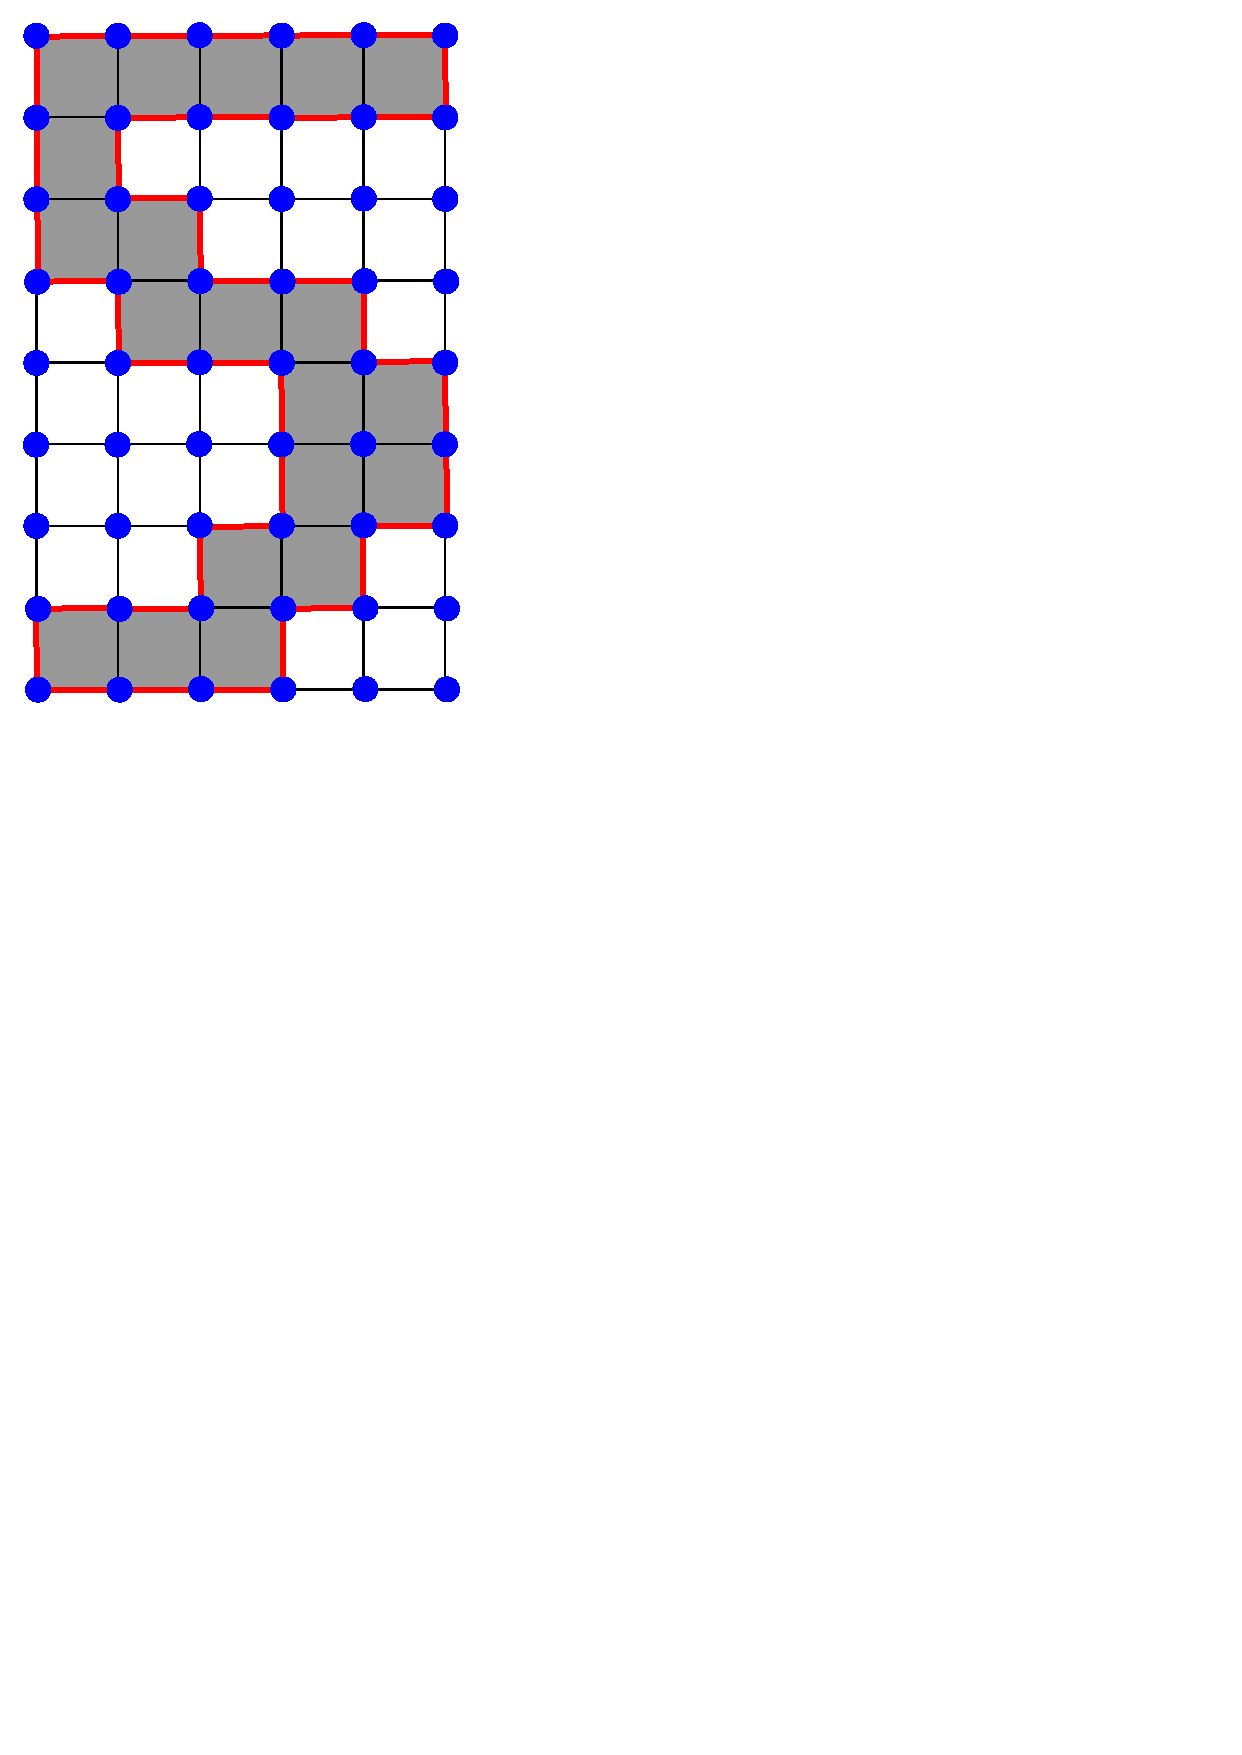
\includegraphics[scale=0.5, trim = 0mm 170mm 130mm 0mm, clip]{imgs/five}}
\caption{Образец с сеткой.}
\end{figure}
Несмотря на очевидную простоту задачи, присутствуют некоторые сложности. 
Как, например, продолжать обход графа в ситуации, показанной на рис. \ref{where}?
\begin{figure}[H]
\centering
{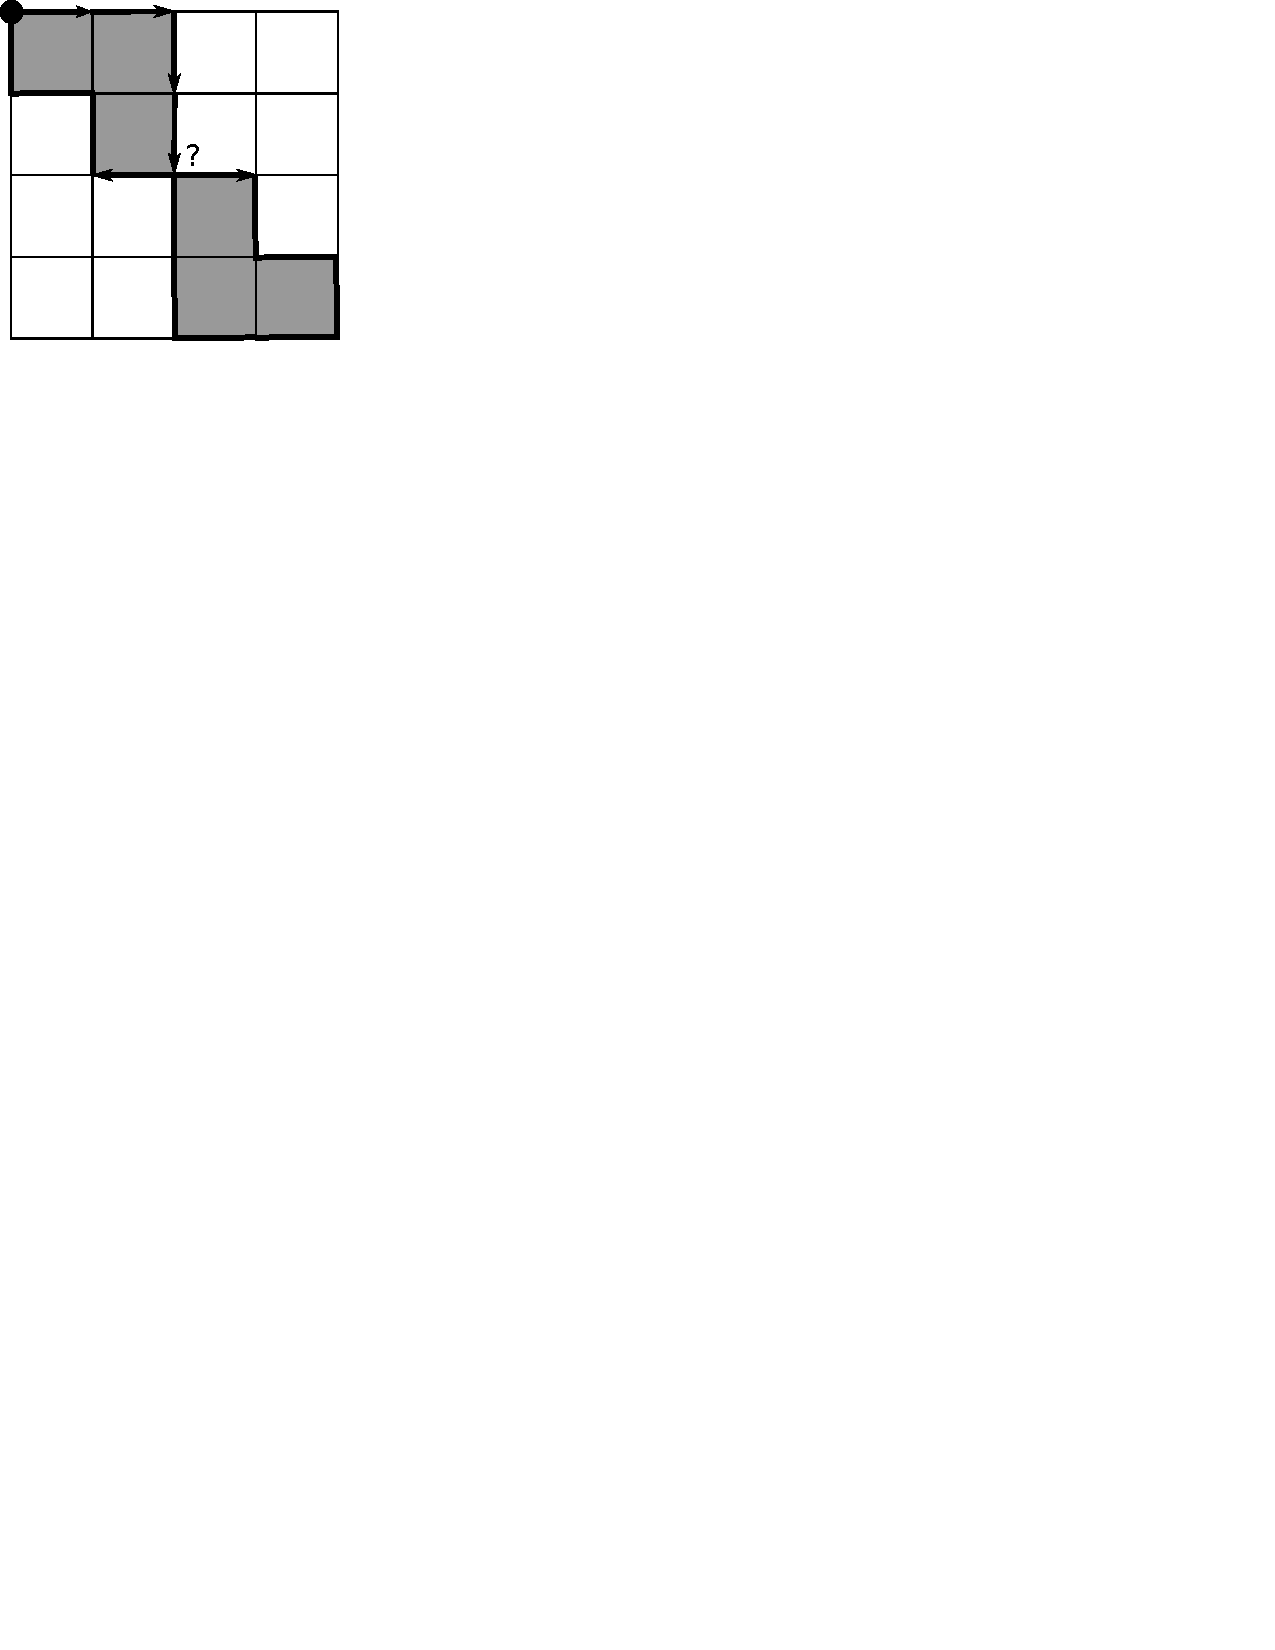
\includegraphics[scale=0.9, trim = 0mm 215mm 155mm 0mm, clip]{imgs/where}}
\label{where}
\caption{Сложная ситуация при обходе.}
\end{figure}
В итоге, контур символа можно получить начав обход картинки из любой вершины на внешнем контуре 
и прийдя к начальной же вершине. Однако, на данный момент мы имеем не контур, а всего лишь вершины построенного графа.
Сопоставив каждой вершине её естественные координаты (строка, столбец), получаем замкнутый контур (который далее,
для ускорения работы, аппроксимируется полигоном с меньшим количеством вершин).

\subsubsection*{Подсчет особенностей}
\par Дескрипторы Фурье для замкнутой кривой -- это коэффициенты разложения 
специально построенной для этой кривой функции в ряд Фурье (подробности см. в \cite{zahn}. Эти коэффициенты инварианты относительно 
операций перемещения, растяжения и, опционально, поворота, что позволяет сделать довольно хорошее сравнение образца
распознавания с эталонами.

Для замкнутой полигональной кривой дескрипторы высчитываются по формулам:
\[
  a_n = -\frac{1}{n\pi}\sum_{k=1}^{m}\bigtriangleup\phi_k\sin(\frac{2\pi n l_k}{L}),~
  b_n = \frac{1}{n\pi}\sum_{k=1}^{m}\bigtriangleup\phi_k\cos(\frac{2\pi n l_k}{L}),
\]
где $n$ - номер коэффициента, $m$ - кол-во вершин в полигоне, $\bigtriangleup\phi_k$ - изменение угла в вершине полигона,
$l_k = \sum_{i=1}^{k}\bigtriangleup l_i$, а $\bigtriangleup l_i$ - длина $i$-ого ребра полигона

Необходимое число дескрипторов варьируется в зависимости от потребностей. Я остановился на числе 25 (итого 50).
\subsubsection*{Распознавание}
\par Итого, символу можно сопоставить вектор дескрипторов. Чтоб сравнить два символа можно посчитать норму разности их 
векторов дескрипторов. А для распознавания была составлена база дескрипторов для трех различных шрифтов; в качестве 
результата распознавания выдается символ, который лучше всего сравнился с образцом.

\begin{codebox}
  \Procname{$\proc{RecognizeSymbol(S)}$}
  \li \Comment $S$ - образец
  \li
  \li \Comment Выделение контура
  \li $Contour = \proc{GetContour(S)}$
  \li
  \li \Comment Подсчет дескрипторов
  \li $Descriptors = \proc{CalcDescriptors($Contour$)}$
  \li
  \li \Comment Поиск наилучшего символа в базе
  \li $BestNorm \gets \infty, BestSymbol \gets \varnothing$
  \li \For $(BSymbol, BDescriptors) \in SymbolsBase$
    \li \Do
    \li	\If $||BDescriptors - Descriptors|| < BestNorm$
    \li \Then
    \li $BestNorm \gets ||BDescriptors - Descriptors||$
    \li $BestSymbol \gets BSymbol$
    \li \End
  \li \End
  \li \Return $BestSymbol$
\end{codebox}

\section{Извлечение кусочно-линейных графических элементов}
\subsection{Задача}
Основная часть изображения химической структуры -- связи между атомами. Большинство связей изображаются с помощью
отрезков, который располагаются по-особенному и могут соединяться (в соединении распологается атом углерода). В мою 
задачу входило нахождение всех отрезков на картинке, в которой уже нет букв.

\begin{figure}[H]
\centering
{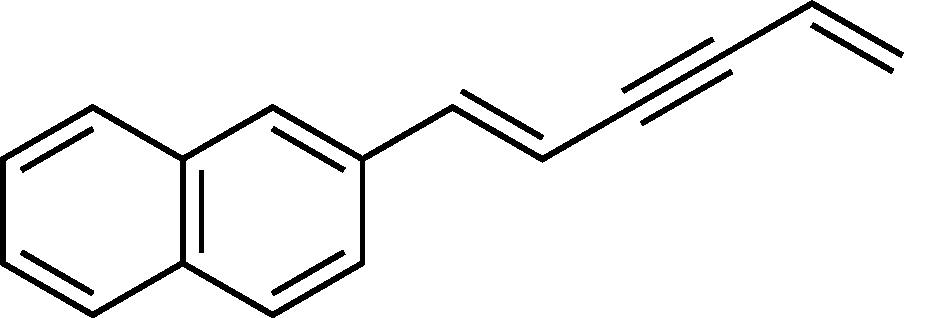
\includegraphics[scale=0.3, trim = 0mm 0mm 0mm 0mm, clip]{imgs/graphics}}
\caption{Связи в изображении молекулы}
\end{figure}


\subsection{Решение}
Для решения задачи был придуман оригинальный метод:

\begin{enumerate}
 \item Сначала к картинке применялся фильтр утоньшения (см. \cite{cychosz}), после которого 
       толщина связи становилась равной 1. 
 \item Затем разрывались сложные (в которых соединяется более двух отрезков) цепочки: если у 
       пиксела есть не меньше 3 черных пиксела 
       в 8-соседях, то этот пиксел становится белым.
 \item Потом картинка сегментировалась, и каждая простая цепочка (ломаная) подвергалась векторизации.
\end{enumerate}

\begin{figure}[H]
\centering
\subfloat[Утоньшенная картинка с разорванными сложными цепочками]{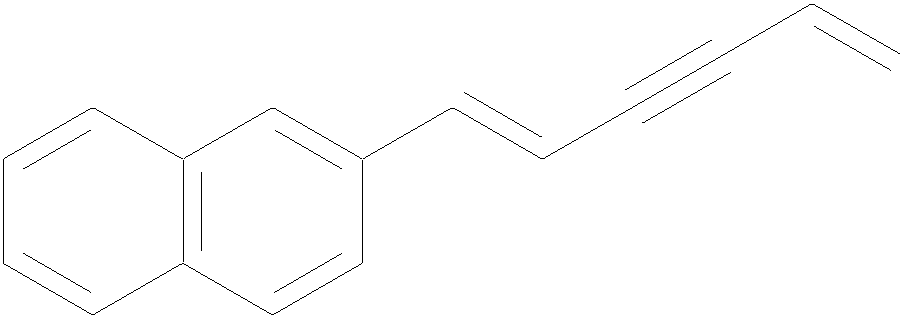
\includegraphics[scale=0.4, trim = 0mm 0mm 0mm 0mm, clip]{imgs/decornered}} \\
\subfloat[Векторизованные отрезки]{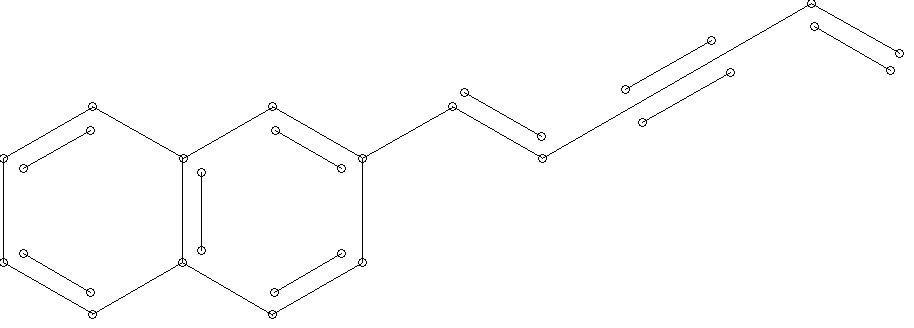
\includegraphics[scale=0.4, trim = 0mm 0mm 0mm 0mm, clip]{imgs/graph_begin}}
\caption{Процесс работы метода.}
\end{figure}


\begin{thebibliography}{4}

\bibitem{ocr}
  Ř Due Trier, AK Jain, T Tax, 
  \emph{Feture extraction methods for character recognition - a survey},
  Pattern recognition, 1996

\bibitem{iupac}
  \emph{Graphical Representation Standards For Chemical Structure Diagrams \\ (IUPAC Recommendations 2008)} \\
  \url{http://www.iupac.org/publications/pac/80/2/0277/}

\bibitem{zahn}
  Charles T. Zahn \& Ralph Z. Roskies,
  \emph{Fourier Descriptors for Plane Closed Curves},
   IEEE Transactions on computers, Vol. c-21, No. 3, march 1972

\bibitem{cychosz}
  Joseph M. Cychosz,
  \emph{"Efficient Binary Image Thinning using Neighborhood Maps"}
  Graphics Gems IV, Academic Press, 1994

\end{thebibliography}

\end{document}
